\documentclass{templateNote}
\usepackage{tcolorbox}
\usepackage{tabularx}
\usepackage{hyperref}
\usepackage{amsmath}
\usepackage{amssymb}
\usepackage{pdflscape}
\usepackage{tikz}
\usepackage{pdfpages}
\usepackage{soul}
\usepackage{media9}
\usepackage{adjustbox}
\usepackage{pdfpages}
\usepackage{enumitem}
\usepackage[spanish,es-noquoting]{babel}

\begin{document}
\linklogoU{https://www.ubiobio.cl/w/}
\linklogoD{https://github.com/NicoGomezM}
\imagenlogoU{img/logo-ubb-txt-face.png}
\imagenlogoD{img/logoNGMFormal_sinF.png}
\titulo{Laboratorio 6: MIPS Assembly Language Programming}
\asignatura{Laboratorio Arquitectura de Computadores}
\autor{
    Nicolás \textsc{Gómez Morgado}
}

\portada
\margenes

\section{Actividades}
\subsection{SPIM}
\noindent Instale la aplicación PCSPIM en PC de laboratorio. Este software está disponible desde Moodle, debe descargar también los códigos assembler adjuntos.
\begin{enumerate}[label=\alph*)]
    \item Averigüe qué es una directiva y cuál es el propósito de las directivas .data, .asciiz, .byte y . text. 
    
    Una directiva es una instrucción que le dice al ensamblador que realice una tarea específica. Las directivas son instrucciones que no se traducen en instrucciones de máquina, sino que le dicen al ensamblador cómo ensamblar el código. A su vez las directivas .data, .asciiz, .byte y .text son directivas que se utilizan para definir el tipo de datos que se van a utilizar en el programa. Por ejemplo:
    \begin{center}
        \begin{tabular}{|c|c|}
            \hline
            \textbf{Directiva} & \textbf{Propósito} \\
            \hline
            .data & Define el segmento de datos. \\
            \hline
            .asciiz & Define una cadena de caracteres. \\
            \hline
            .byte & Define un byte. \\
            \hline
            .text & Define el segmento de texto. \\
            \hline
        \end{tabular}
    \end{center}
    \item Ejecute el simulador y cargue el programa “1.s”. Identifique el “segmento de datos” (captura del segmento de datos).
    
    En el programa la zona del segemnto de datos se puede identificar como el lugar donde aparecen los titulos \textbf{DATA}, \textbf{STACK} y \textbf{KERNEL DATA}. Como se muestra en las siguientes capturas: 

    \begin{figure}[H]
        \centering
        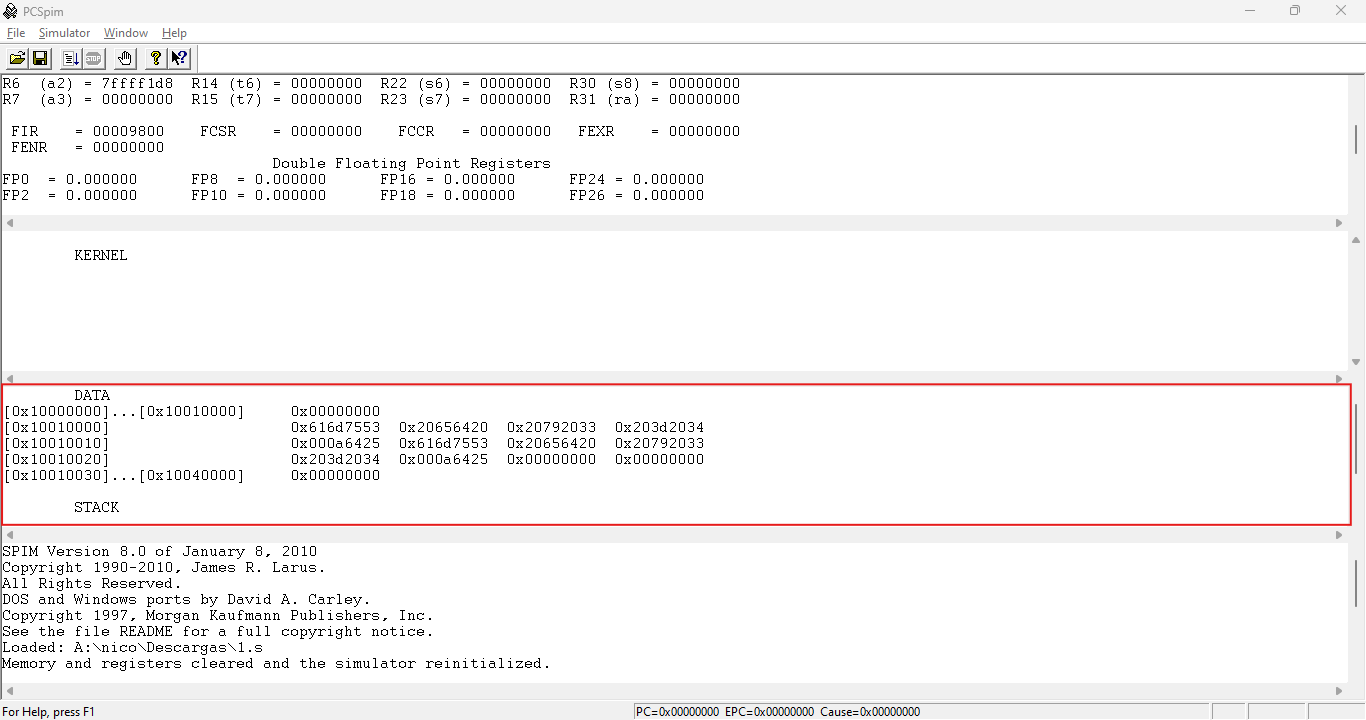
\includegraphics[width=1\textwidth]{img/img1.png}
        
\includegraphics[width=1\textwidth]{img/img2.png}
    \end{figure}

    \item Identifique en qué lugar de la memoria se almacena el arreglo de bytes. Explicite la dirección de memoria de cada byte (utilice una calculadora online para la conversión de base: Suma de 3 y 4 = \%d\textbackslash n).
    
    Las direcciones de memoria donde se almacena el arreglo de bytes se pueden identificar en la siguiente zona:
    \begin{figure}[H]
        \centering
        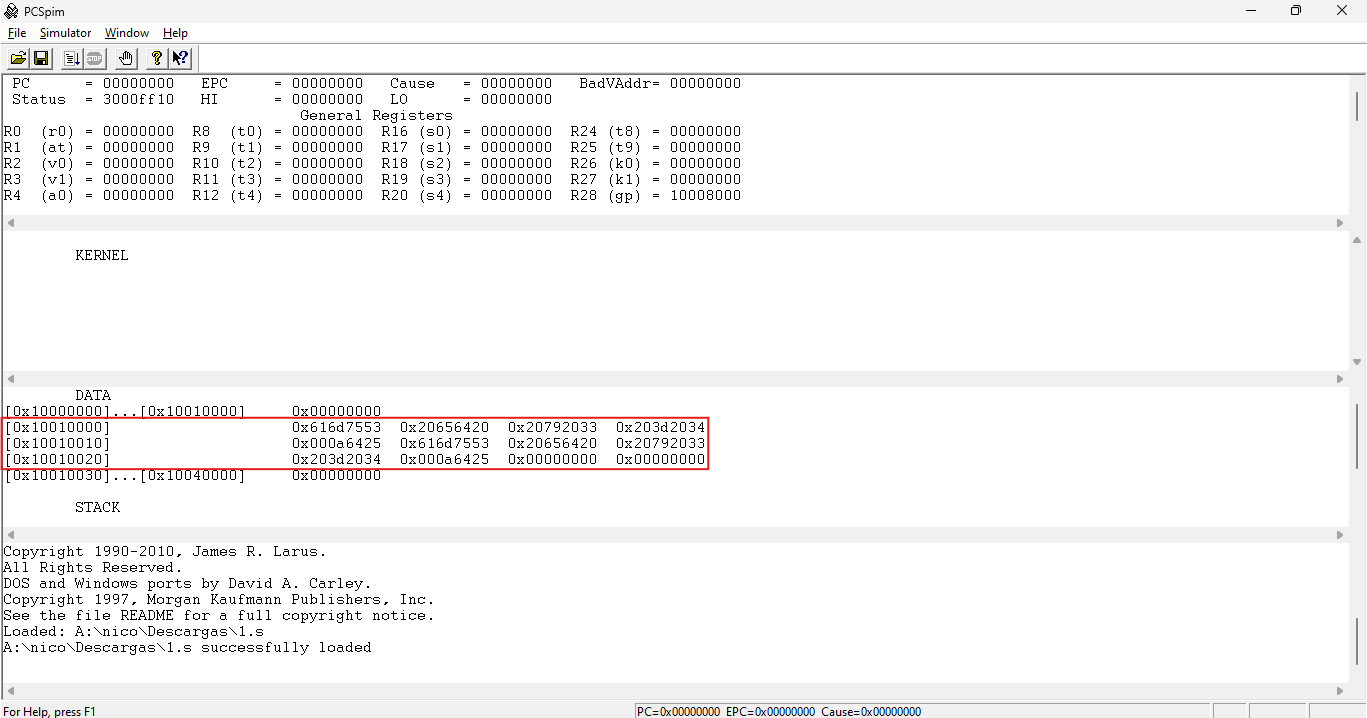
\includegraphics[width=1\textwidth]{img/img3.png}
    \end{figure}
    Siendo estas direcciones:
    \begin{itemize}
        \item 0x10010000
        \item 0x10010010
        \item 0x10010020
        \\Mas especificamente:
        \begin{itemize}
            \item 0x10000000: 53 = 'S'
            \item 0x10000001: 75 = 'u'
            \item 0x10000002: 6d = 'm'
            \item 0x10000003: 61 = 'a'
            \item 0x10000004: 20 = ' '
            \item 0x10000005: 64 = 'd'
            \item 0x10000006: 65 = 'e'
            \item 0x10000007: 20 = ' '
            \item 0x10000008: 33 = '3'
            \item 0x10000009: 20 = ' '
            \item 0x1000000A: 79 = 'y'
            \item 0x1000000B: 20 = ' '
            \item 0x1000000C: 34 = '4'
            \item 0x1000000D: 20 = ' '
            \item 0x1000000E: 3d = '='
            \item 0x1000000F: 20 = ' '
            \item 0x10000010: 25 = '\%'
            \item 0x10000011: 64 = 'd'
            \item 0x10000012: 0a = '\textbackslash n'
            \item 0x10000013: 00 = Final cadena de caracteres.
        \end{itemize}
    \end{itemize}

    
    \item Busque online una tabla ASCII. Identifique en memoria de datos la frase “Suma de 3 y 4 = \%d\textbackslash n”.
    \begin{center}
        https://www.chileoffshore.com/es/toolkits/basic-conversion/ascii-to-hexa    
    \end{center}

    La frase transformada seria la siguiente: \\
    53756D61206465203320792034203D2025645C6E. \\
    La cual divida en 8 caracteres por sector, se obtiene lo siguiente:
    \begin{itemize}
        \item 53 75 6D 61 
        \item 20 64 65 20
        \item 33 20 79 20 
        \item 34 20 3D 20
        \item 25 64 5C 6E
    \end{itemize}

    Estos caracteres de la frase se giran, obteniendo lo siguiente:

    \begin{itemize}
        \item 61 6D 75 53 = 0x616d7553 = 'Suma'
        \item 20 65 64 20 = 0x20656420 = ' de '
        \item 20 79 20 33 = 0x20792033 = '3 y '
        \item 20 3D 20 34 = 0x203D2034 = '4 = '
        \item 6E 5C 64 25 = 0x6E5C6425 = '\%d\textbackslash n'
    \end{itemize}


    \item Averigüe y concluya qué ordenamiento de datos emplea SPIM (Little Endian o Big Endian).
    
    SPIM emplea el ordenamiento de datos Little Endian, ya que en este ordenamiento los bytes menos significativos se almacenan en las direcciones de memoria más bajas, mientras que los bytes más significativos se almacenan en las direcciones de memoria más altas.

    \item Cargue el programa “2.s”. identifique en qué dirección de memoria se inicia el segmento de instrucciones.

    El programa 2.s inicia el segmento de instrucciones en la dirección de memoria \textbf{0x00400000}.
    
    \item Identifique qué significado posee la etiqueta main.

    La etiqueta main es donde se describen las instrucciones que se ejecutarán al inicio del programa. Es el punto de entrada del programa.

    \item Explique el propósito de la directiva align. Para ello cambie el valor de 2 a 4 de cualquiera de las declaradas y observe cambios (editar con procesador de texto).     

    La directiva .align se encarga de alinear la dirección de memoria de la siguiente instrucción a un múltiplo de 2. Si se cambia el valor de 2 a 4, la dirección de memoria de la siguiente instrucción se alineará a un múltiplo de 4.
\end{enumerate}

\newpage
\begin{tcolorbox}
    \textbf{Las primeras imagenes se tomaron sin reiniciar el programa, y por falta de tiempo se dejaron asi, pero solo son una duplicacion de la respuesta solicitada}
\end{tcolorbox}

% \newpage  
\subsection{Entrega}
\begin{enumerate}[label=\alph*]
    \item Documentar cada una de las acciones antes señaladas. Es de exclusiva responsabilidad del estudiante respetar el formato de entrega de esta guía. El formato de entrega debe ser en .pdf, capturas legibles, recortadas y centradas, el nombre del archivo debe contener su nombre y apellido (Laboratorio\_6\_Nombre\_Apellido). Todas las actividades deben ser entregadas (subidas) a la plataforma digital en las fechas establecidas. Por cada hora de atraso, se descontará 1 pto.
\end{enumerate}

\end{document}